\section{Control system design}

\subsection{Problem a}

The PD transfer function is of the form
\begin{align*}
    H_{pd}(s) &= K_{pd}(1+T_d s)/(1+T_f s) \\
              &= K_{pd}(1+T s)/(1+\alpha T s)
\end{align*}

Where $T_d = T$ in order to cancel the systems pole factor $(Ts + 1)$, and $T_f = \alpha T_d = \alpha T$. We set $K_{pd} = 0.8, \alpha = 0.1$. Figure INSERT contains the bode plot of the system $H(s) = H_{ship}(s)H_{pd}(s)$, with the phase margin Pm at 48.3 degrees, and crossover angular frequency at 0.104 rad/s.

\begin{figure}[ht]
    \centering
    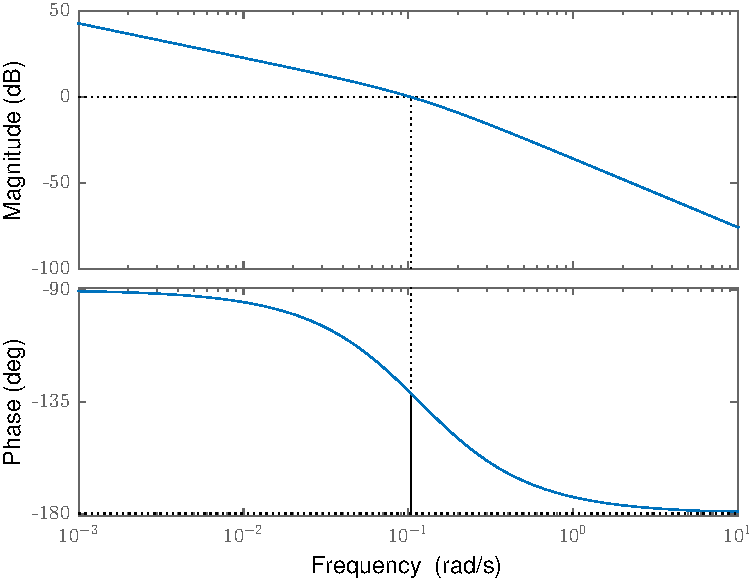
\includegraphics[width=0.5\textwidth]{images/3a-bode_and_phasemargin}
    \caption{Bode - and phase margin plot}
    \label{fig:3a-bode_and_phasemargin}
\end{figure}

\subsection{Problem b}
As shown in \cref{fig:3b-psi_and_rudder}, the autopilot functions with only measurement noise.

\begin{figure}[ht]
    \centering
    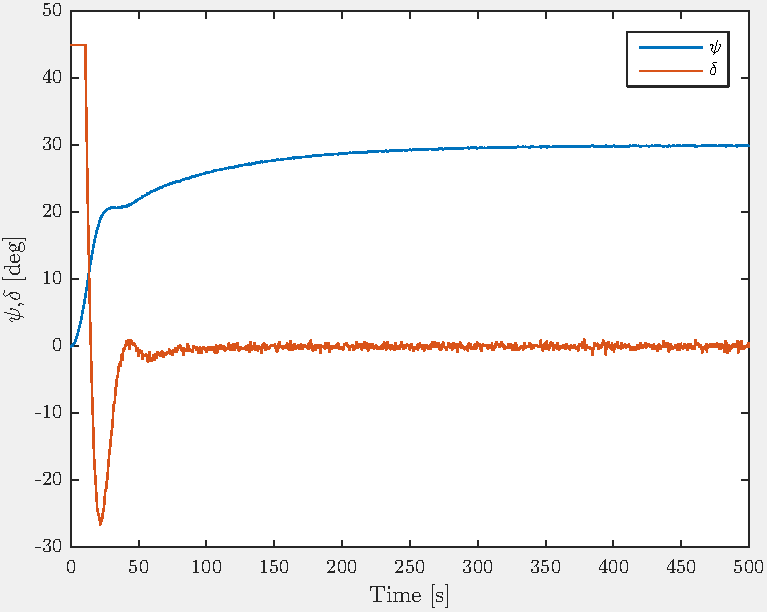
\includegraphics[width=0.5\textwidth]{images/3b-psi_and_rudder}
    \caption{Compass angle, $\psi$, and rudder angle, $\delta$}
    \label{fig:3b-psi_and_rudder}
\end{figure}

\subsection{Problem c}
As shown in \cref{fig:3b-psi_and_rudder_w_current}, the autopilot functions somewhat but has a stationary deviation as expected.

\begin{figure}[ht]
    \centering
    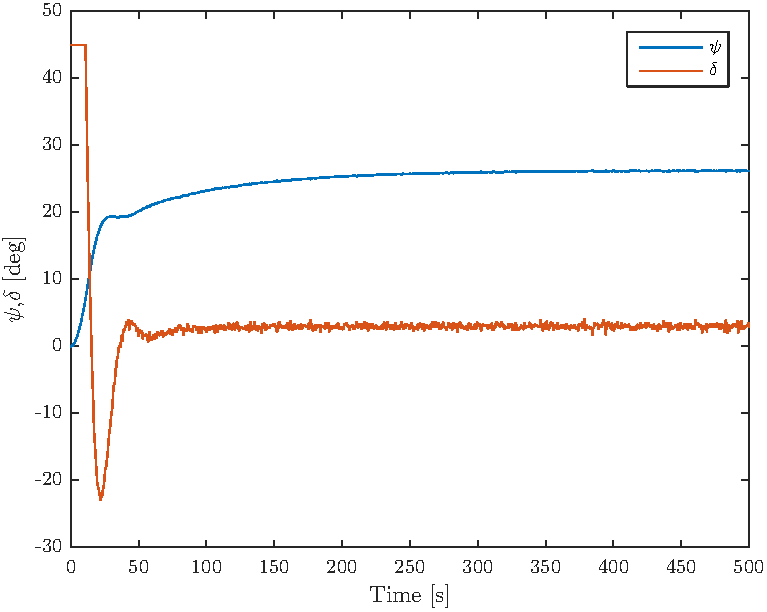
\includegraphics[width=0.5\textwidth]{images/3c-psi_and_rudder_w_current}
    \caption{Compass angle, $\psi$, and rudder angle, $\delta$, with current disturbance}
    \label{fig:3b-psi_and_rudder_w_current}
\end{figure}

\subsection{Problem d}
As shown in \cref{fig:3b-psi_and_rudder_w_waves}, the autopilot functions somewhat but with unacceptable high frequent noise that would strain the motors of the ship.

\begin{figure}[ht]
    \centering
    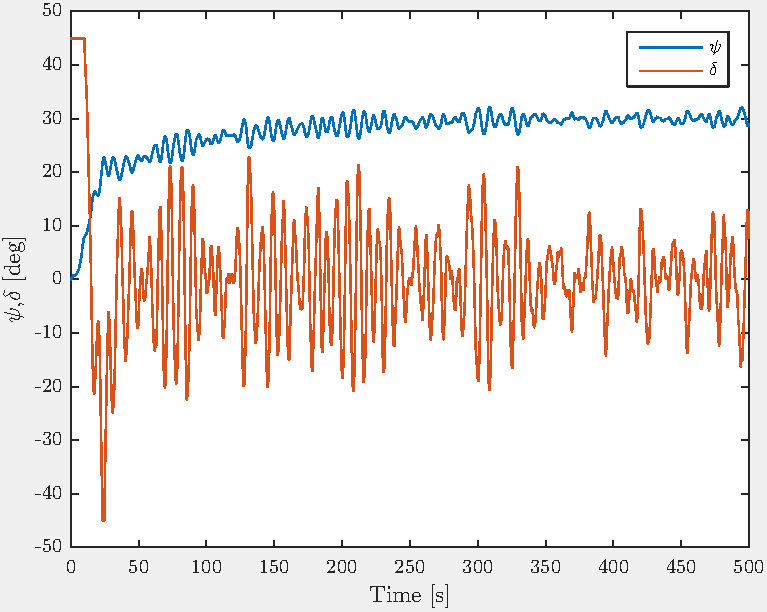
\includegraphics[width=0.5\textwidth]{images/3d-psi_and_rudder_w_waves}
    \caption{Compass angle, $\psi$, and rudder angle, $\delta$, with wave disturbance}
    \label{fig:3b-psi_and_rudder_w_waves}
\end{figure}